\documentclass[border=2pt]{standalone}
\usepackage{tikz}
\usetikzlibrary{quotes,angles}
\usepackage{amsmath}

\begin{document}

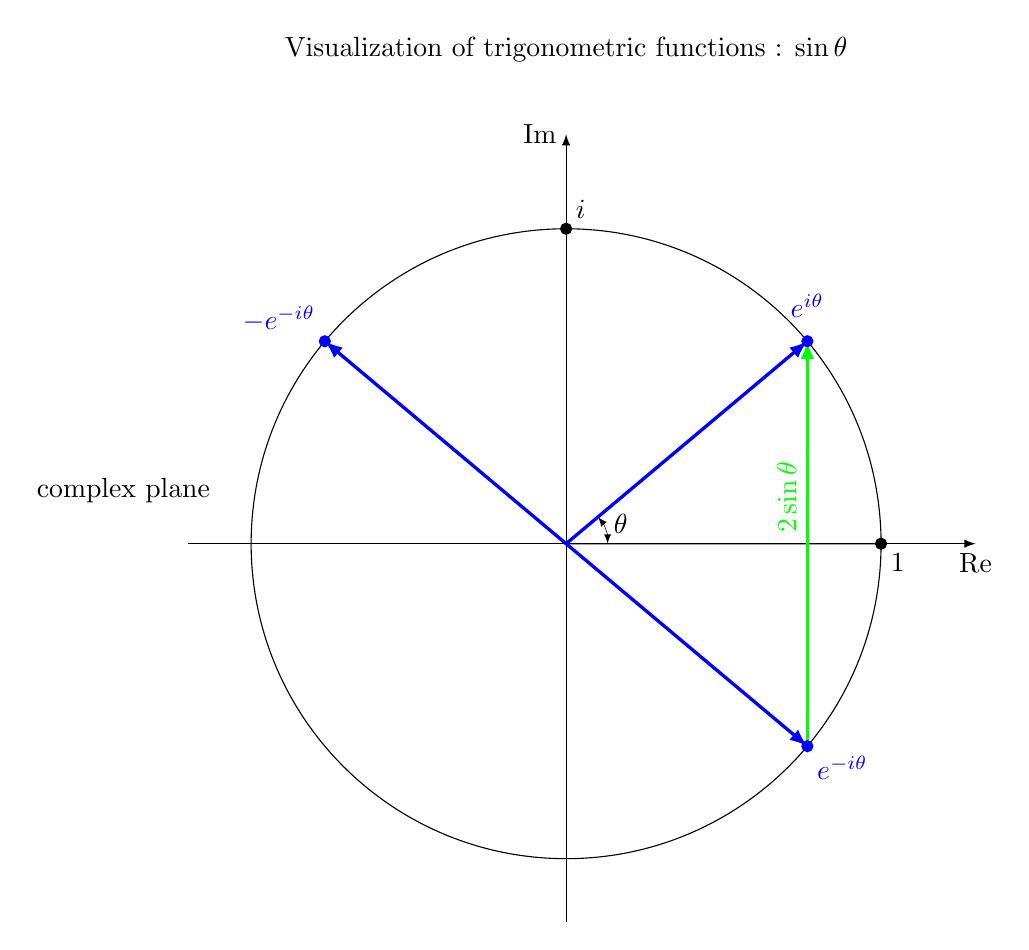
\begin{tikzpicture}[scale=4]

% Draw x and y axis lines
\draw [->,>=latex] (-1.2,0) -- (1.30,0) node [below] {$\mathrm{Re}$};
\draw [->,>=latex] (0,-1.2) -- (0,1.30) node [left] {$\mathrm{Im}$};
\node[above left] at (-1.1, 0.1) {complex plane};
\filldraw[black] (1,0) circle (0.5pt) node[below right] {$1$} ;
\filldraw[black] (0,1) circle (0.5pt) node[above right] {$i$} ;
\node[above] at (0.0,1.50) {Visualization of trigonometric functions : $\sin \theta$};

% Draw a circle at the origin of radius 1
\draw (0,0) circle (1);

\pgfmathsetmacro{\angle}{40}


\draw
  (1,0) coordinate (a) 
  -- (0,0) coordinate (b) 
  -- ( {cos(\angle)}, {sin(\angle)} ) coordinate (c) 
  pic["$\theta$", draw=black, very thin, <->,>=latex, angle eccentricity=1.4, angle radius=15]
  {angle=a--b--c};


\draw [color=blue, very thick, ->,>=latex] (0,0) -- ( {cos(\angle)}, {sin(\angle)} ) ;
\draw [color=blue, very thick, ->,>=latex] (0,0) -- ( {cos(\angle)},-{sin(\angle)} ) ;
\draw [color=blue, very thick, ->,>=latex] (0,0) -- (-{cos(\angle)}, {sin(\angle)} ) ;

\draw [color=green, very thick, ->,>=latex] ( {cos(\angle)},-{sin(\angle)} ) --  node[above right, rotate=90] {$2\sin\theta$} ( {cos(\angle)}, {sin(\angle)} ) ;

\filldraw[blue] ( {cos(\angle)}, {sin(\angle)} ) circle (0.5pt) node[color=blue, above=5pt] {$e^{i\theta}$} ;
\filldraw[blue] (-{cos(\angle)}, {sin(\angle)} ) circle (0.5pt) node[color=blue, above left ] {$-e^{-i\theta}$} ;
\filldraw[blue] ( {cos(\angle)},-{sin(\angle)} ) circle (0.5pt) node[color=blue, below right] {$e^{-i\theta}$} ;






\end{tikzpicture}

\end{document}

